% The literature review is an essential requirement of any academic project. A comprehensive review of the literature will provide background to the project and should be used to inform and guide the research to be undertaken for your project, as well as help guide any software solution. It also establishes that what you have done is the result of academic study, rather than an unfounded whim. This section can build upon the literature you investigated in assessment 1 for the proposal document. You should use the feedback from your supervisor to improve upon the final version. 

% It may be helpful to break up this chapter into sections, with each focused on a different topic or aspect of the project.

%This should be a coherent, critical evaluation of relevant academic literature with clear linkage to your project. You may use and build upon the brief literature survey from your project proposal (which you must reference). You should be aiming to produce a literature review that clearly identifies the area of interest your project sits in, and how it aligns with/builds upon the published work. The project aims and objectives should also be revisited here in its own sub-section.

% goal ~4.5k words
% actual 4147 words

% setup the literature review with a short intro on what computer vision and its subfields are

Computer Vision is a subfield of Artificial Intelligence that has for goal to give machines the sense of vision, or in other words, the ability to perceive and recognise objects. Within Computer Vision there are many more subfields, such as object detection, object segmentation, human pose estimation, motion detection, etc. These are the methods I will be looking at in this review.

\section{Object Detection}
    The ability to identify and locate objects in an image or video is one of the fundamental objectives of computer vision. To improve the accuracy and efficiency of object detection, many methods have been developed over time. Histogram of gradients (HOG) and Haar cascades are examples of conventional methods. The Haar cascades, developed by Paul Viola and Michael Jones, use a series of fundamental classifiers to identify objects based on features such as edges and lines that are derived from integral images. Their capacity to recognise faces has earned them particular notoriety \citep{viola2001rapid}. HOG descriptors, which are helpful for recognising pedestrians and other things with different forms, were developed by Navneet Dalal and Bill Triggs. They function by first dividing an image into small cells, then calculating the gradient orientation histogram for each of those cells, and finally normalising the output \citep{dalal2005histograms}.\\

    \begin{figure}[htbp]
        \centering
        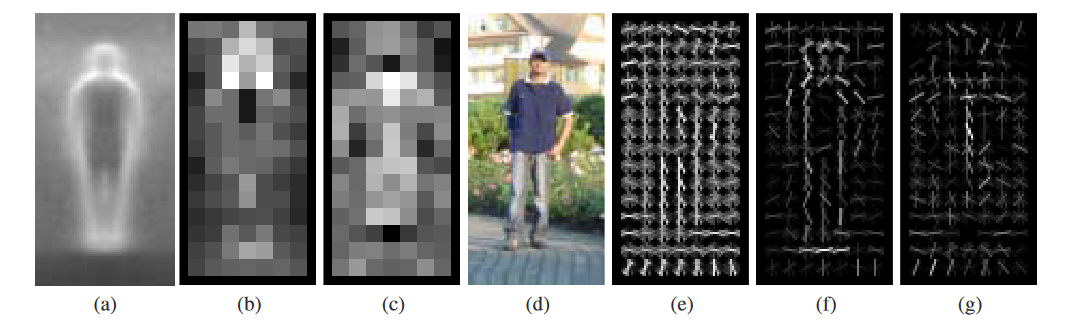
\includegraphics[width=0.99\textwidth]{figures/HOG.png}
        \caption{Navneet Dalal and Bill Triggs' HOG detectors cue mainly on silhouette contours (especially the head, shoulders and feet). The most active blocks are centred on the image background just outside the contour. (a) The average gradient image over the training examples. (b) Each “pixel” shows the maximum positive SVM weight in the block centred on the pixel. (c) Likewise for the negative SVM weights. (d) A test image. (e) It’s computed R-HOG descriptor. (f,g) The R-HOG descriptor weighted by respectively the positive and the negative SVM weights. \citep{dalal2005histograms}}
        \label{fig:HOG}
    \end{figure}

    Deep learning algorithms have considerably improved the detection of objects. Region-Based Convolutional Neural Networks, or R-CNN, by Ross Girshick et al., resorted to a two-step process of generating region proposals and classifying each proposal using a CNN. While this gave better accuracy in detection, it added a large computational cost \citep{girshick2014rich}. Fast R-CNN by Ross Girshick does this with even better performance by integrating the recommendation of regions and classification into a single network. There will be one RoI pooling layer to pool the features of each proposal \citep{girshick2015fast}. Faster R-CNN by Shaoqing Ren et al. incorporates region proposal networks, or RPNs for short, that share some convolutional layers with the detection network to provide near cost-free region proposals, thus speeding up the detection \citep{ren2015faster}. \\

    \begin{figure}[htbp]
        \centering
        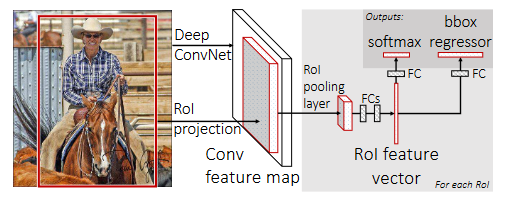
\includegraphics[width=0.80\textwidth]{figures/Fast_R-CNN.png}
        \caption{Fast R-CNN architecture.\citep{girshick2015fast}}
        \label{fig:FastRCNN}
    \end{figure}

    Single Shot MultiBox Detector (SSD) by Wei Liu et al. bypass region proposal completely and use a single network to predict object classes and bounding boxes directly from feature maps at all scales. It goes in direct balance with speed and accuracy for the real-time application \citep{liu2016ssd}. Along this line, Tsung-Yi Lin et al. form the above class imbalance problem in the dense object detection task to the newly introduced function Focal Loss in RetinaNet. This is done by down-weighting the loss of the well-explained model instances to give the most focus to the hard-to-classify instances \citep{lin2017focal}.\\
    
    These methods present the evolution of object detection techniques from traditional ones, based on handcrafted features, to the modern deep learning-based framework with the power of Convolutional Neural Networks. This particular feature is strong in one visual function or another, and choice in using a method can often come down to the specifics of the application requirements, such as speed, accuracy, and computational resources.

\section{Methods of Segmentation}
    Image segmentation is considered one of the most prominent tasks done in the field of computer vision. The process can be defined as partitioning a given image into a number of segments or regions, where every part represents some meaningful portion of the original image. Several schemes have been developed through the years to achieve perfect and efficient segmentation. The classical ones include thresholding, edge detection, and region-based segmentation. Thresholding: This type of simple segmentation simply takes a greyscale image and the threshold values to convert the image into a binary image. All pixels that have intensity values larger than the threshold are considered as foreground, and those with lower intensity values are classified under background. The technique of this kind basically works for those images that have huge differences in the values of intensity between objects and their background \citep{otsu1975threshold}. Edge detection methods, exemplified by the classic one—Canny edge detector—are designed to identify object boundaries in an image by the detection of intensity discontinuities. They are used in applications where it can segment objects having well-defined edges. One of the most used was that developed by John Canny, known as the Canny edge detector, for its ability to detect edges with low error rates and good localisation \citep{canny1986computational}. Methods for region-based image segmentation group pixels together with certain similar properties. The major methods are region growing and region splitting and merging. Region growing does the segmentation from user-specified starting points by picking neighboring pixels that meet the specified criteria. Region splitting and merging divide an image into local regions and then combine them into groups using measures of similarity \citep{adams1994seeded}.\\

    \begin{figure}[htbp]
        \centering
        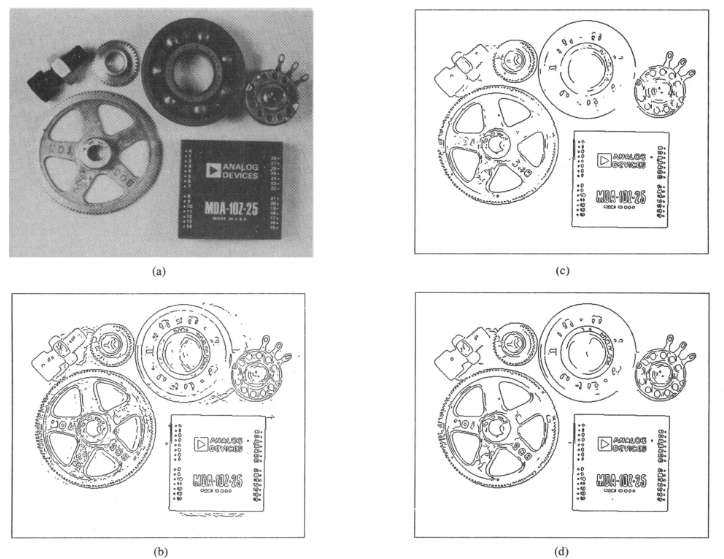
\includegraphics[width=0.49\textwidth]{figures/canny.png}
        \caption{(a) Parts image, 576 by 454 pixels. (b) Image thesholded at T,. (c) Image thresholded at 2 T,. (d) Image thresholded with hysteresis using both the thresholds in (a) and (b). \citep{canny1986computational}}
        \label{fig:canny}
    \end{figure}

    Deep learning techniques have significantly enhanced image segmentation procedures. Fully Convolutional Networks are one kind of neural network designed explicitly for pixel-wise prediction tasks by Jonathan Long et al. In general, an FCN is an extension of the traditional CNNs; it replaces fully connected layers with convolutional layers so that the network outputs a segmentation map of the same size as the input image. It increased the accuracy of semantic segmentation to a large extent \citep{long2015fully}. Probably the most popular biomedical image segmentation architecture is the U-Net introduced by Olaf Ronneberger et al. The U-Net represents a network with an encoder-decoder architecture that provides high-resolution features from the encoder, which are concatenated with upsampled features from the decoder through skip connections. This design enables retaining spatial information and improves segmentation accuracy \citep{ronneberger2015u}. Mask R-CNN, introduced by Kaiming He et al., extends Faster R-CNN with an added branch for predicting a segmentation mask on each Region of Interest (RoI). While Faster R-CNN just localises the object, the method can do instance segmentation—in that each object instance is segmented on its part. Widespread adoption has taken place due to the accuracy and versatility of Mask R-CNN \citep{he2017mask}. The DeepLab was developed by Liang-Chieh Chen et al. and uses atrous or dilated convolutions to stride contextual information at multiple scales without losing resolution. DeepLab also integrates Conditional Random Fields that help refine segmentation borders, enabling it to effectively segment complex-shaped and scale-varying objects \citep{chen2017deeplab}.\\

    \begin{figure}[htbp]
        \centering
        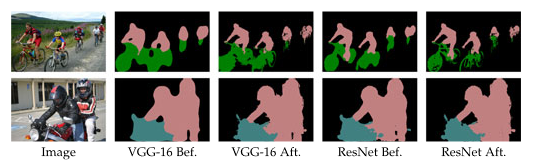
\includegraphics[width=0.99\textwidth]{figures/deeplab.png}
        \caption{DeepLab results based on VGG-16 net or ResNet-101 before and after CRF. The CRF is critical for accurate prediction along object boundaries with VGG-16, whereas ResNet-101 has acceptable performance even before CRF.\citep{chen2017deeplab}}
        \label{fig:deeplab}
    \end{figure}

    The methods include traditional heuristic approaches to image segmentation and more advanced and deep learning-based frameworks that are empowered by neural networks. Each of the methods will have a share in strong and weak points and be more suitable for certain applications than others depending on the accuracy required, computational efficiency, and the type of complexity involved in the segmentation.
    

\section{Human Pose Estimation (HPE)}
    Human pose estimation is a process for detecting and tracking the location of key body joints in images or videos; it is thus of paramount importance in the field of computer vision. This has been applied to motion capture, activity recognition, human–computer interaction, and other areas. Two traditional solutions are pictorial structures and deformable part models. Pictorial structures model a human body as a collection of rigid parts connected by flexible joints. Each part is modeled using a template, and configuration of parts is optimised to fit the observed image. This framework, thanks to Felzenszwalb and Huttenlocher has been quite successful in detecting human poses in static images \citep{felzenszwalb2005pictorial}. Deformable Part Models generalise pictorial structures to allow for deformation of parts relative to each other. Felzenszwalb et al.'s method represents the object class by a mixture of templates, each capturing appearance and pose variations. DPMs have been used in many applications involving object detection and human pose estimation \citep{felzenszwalb2009object}.\\

    \begin{figure}[htbp]
        \centering
        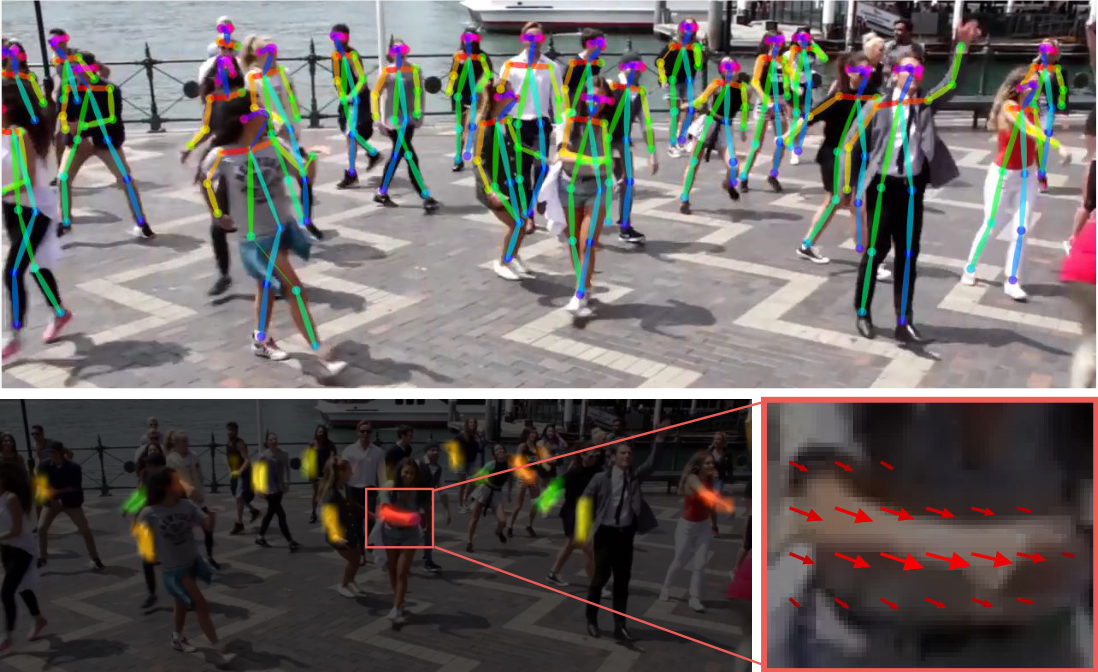
\includegraphics[width=0.49\textwidth]{figures/multipose.png}
        \caption{Top: Multi-person pose estimation. Body parts belonging to the same person are linked. Bottom left: Part Affinity Fields (PAFs) corresponding to the limb connecting right elbow and right wrist. The color encodes orientation. Bottom right: A zoomed in view of the predicted PAFs. At each pixel in the field, a 2D vector encodes the position and orientation of the limbs. \citep{cao2017realtime}}
        \label{fig:multipose}
    \end{figure}

    Deep learning-based methods have greatly advanced human pose estimation. Employing a sequence of convolutional networks to iteratively predict the locations of body joints, the Convolutional Pose Machines method has already shown very accurate results. In each stage of this network, it is expected to refine the prediction in the previous stage, hence improving the accuracy in pose estimation iteratively \citep{wei2016convolutional}. The Stacked Hourglass Networks by Newell et al. uses symmetric encoder-decoder architecture capturing features at many scales. Such a network is made up of many hourglass modules stacked together, so that it is feasible to perform bottom-up and top-down processing repetitively. This algorithmic approach has achieved a top performance in human pose estimation \citep{newell2016stacked}. OpenPose, developed by Cao et al., is a real-time multi-person pose estimation framework. It uses a two-branch CNN to predict part affinity fields (PAFs) and keypoint locations simultaneously. PAFs encode the spatial relationships between body parts, enabling the network to associate detected keypoints with individual people in the image \citep{cao2017realtime}. PoseNet by Kendall et al. comprises a deep learning framework for estimating human poses from images. This approach uses a CNN to directly predict the 2D coordinates of body joints from an input image and can be end-to-end trained to solve a wide variety of pose estimation tasks. PoseNet has been identified to work quite well in terms of accuracy and to be very robust in very challenging conditions \citep{kendall2015posenet}.\\

    \begin{figure}[htbp]
        \centering
        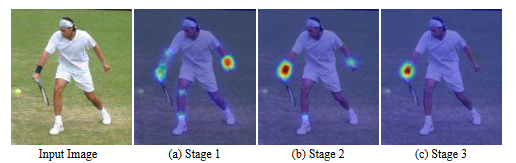
\includegraphics[width=0.75\textwidth]{figures/convPose.png}
        \caption{Here Wei et al. show the increasingly refined estimates for the location of the right elbow in each stage of the sequence. (a) Predicting from local evidence often causes confusion. (b) Multi-part context helps resolve ambiguity. (c) Additional iterations help converge to a certain solution. \citep{wei2016convolutional}}
        \label{fig:convpose}
    \end{figure}
    
    These methods reflect the journey that began with traditional approaches, which relied on handcrafted models for human-pose estimation, to deep-learning-based advanced frameworks exploiting the power of convolutional neural networks. Each approach has its strengths and weaknesses, and very often, the choice of method depends on the kind of application at hand, that is, accuracy, computational efficiency, or the complexity of poses estimated.
    

\section{Motion Tracking}
    One of the big modules of computer vision, motion tracking involves the tracking of a human or any other entity from one frame to another in a video sequence. Major applications include surveillance, sports analysis, and augmented reality. Traditional approaches include optical flow, the Kalman filter, and mean shift. Most of the approaches in use for calculating the motion of an object via optical flow generally make use of the apparent motion of the brightness patterns between consecutive frames. Probably the most famous among these, which assumes constant flow in some small neighbourhood and finds the motion using least squares fitting, is the method proposed by Bruce D. Lucas and Takeo Kanade \citep{lucas1981iterative}. Another popular method is based on the Horn-Schunck algorithm with the smoothness constraint of the flow field in order to cope with noise and discontinuities \citep{chen2016full}. Basically, the Kalman filter is a principle of state estimation for a dynamic system from noisy observations by a recursive algorithm. Since it finds applications in prediction regarding position and velocity for moving objects, it is normally used in motion tracking. Prediction and update are basically the two working steps of the Kalman filter, and the same have been designed efficiently to handle problems regarding real-time tracking \citep{kalman1960new}. Mean shift is a non-parametric feature-space analysis technique applied for finding the maxima of a density function. Applied to motion tracking, it shifts a window iteratively to the area with the highest density of features and uses it to track an object. Thus, this approach is robust against appearance variations of the object and partial occlusions \citep{comaniciu2000real}.\\

    \begin{figure}[htbp]
        \centering
        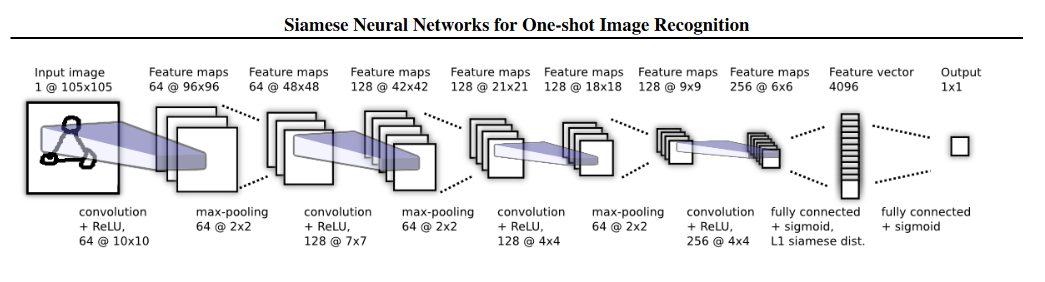
\includegraphics[width=0.99\textwidth]{figures/siamese.png}
        \caption{Best convolutional architecture selected for verification task. Siamese twin is not depicted, but joins immediately after the 4096 unit fully-connected layer where the L1 component-wise distance between vectors is computed \citep{koch2015siamese}}
        \label{fig:siamese}
    \end{figure}

    Deep learning methods have already shown a high improvement in the state-of-the-art performance in motion tracking. RNNs, and especially the LSTM network, conduct motion tracking through modelling temporal dependencies in sequential data. They hence learn how to predict the future positions of objects from their previous trajectories and hence can be applied to track complicated nonlinear motions \citep{hochreiter1997long}. Koch et al. have proposed Siamese networks for application in one-shot learning problems like object tracking. It consists of two identical sub-networks processing two different inputs and returning the similarity score as output. In the case of motion tracking, the Siamese Networks could be trained for the differentiation of target from background and offer robustness under challenging conditions \citep{koch2015siamese}. DeepSORT hybridises the SORT algorithm with a deep appearance descriptor. This approach uses a CNN for extracting features from detected objects and a Kalman filter, which provides motion prediction. By combining both appearance and motion information, this significantly improves not only accuracy but also resilience in tracking \citep{wojke2017simple}. Huang et al. proposed a deep framework called TrackNet for sports tracking. It uses a CNN to predict the heatmap in every frame on the location of the target and further refines these predictions with post-processing. On the other hand, TrackNet was able to track fast-moving targets such as the badminton shuttlecock and tennis ball \citep{huang2019tracknet}. \\

    \begin{figure}[htbp]
        \centering
        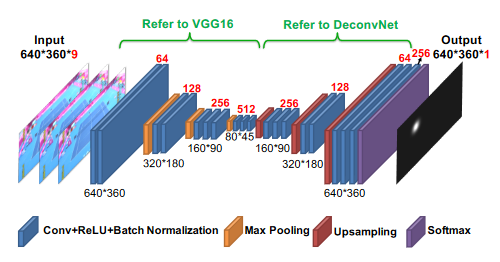
\includegraphics[width=0.6\textwidth]{figures/tracknet.png}
        \caption{The architecture of the proposed TrackNet \citep{huang2019tracknet}}
        \label{fig:tracknet}
    \end{figure}

    These methods very clearly show how far the progress of motion-tracking techniques has moved from more traditional, math-model-based methods to advanced, deep learning-based frameworks that exploit the power of neural networks. But each has its strengths and weaknesses, and often, the choice of the method depends on the specific requirements of the application.

\section{The Cutting Edge of HPE}
    There has been huge progress in HPE, with sophisticated models like YOLO  by Ultralytics and Google's MediaPipe. While both of these frameworks offer very powerful detection and tracking tools for human pose, they differ in approach and capabilities. 
    \begin{figure}[htbp]
        \centering
        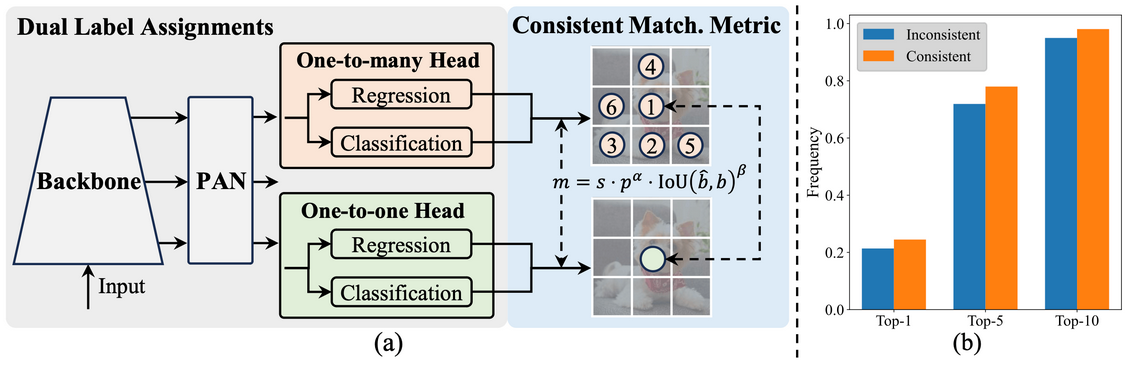
\includegraphics[width=0.8\textwidth]{figures/yolov10arch.png}
        \caption{(a) Consistent dual adddignments for NMS-free training. (b) Frequency of one-to-one assignments in Top-1/5/10 of one-to-many results for YOLOv8-S which employs $\alpha_{o2m}$=0.5 and $\beta_{o2m}$=6 by default. (https://docs.ultralytics.com/models/yolov10/)}
        \label{fig:yolo_arch}
    \end{figure}
    \subsection{YOLO by Ultralytics}
        YOLO stands for 'You Only Look Once,' referring to a family of real-time object detection models that have evolved significantly since their appearance. The newest version, YOLOv10, will raise the power from its predecessors to even more performance and versatility. Joseph Redmon et al. developed the first model for YOLO. It introduced a single unified architecture processing full images in pass-through, very fast \citep{redmon2016you}. Batch Normalisation, Anchor Boxes, and Dimension Clusters improve YOLOv2 \citep{redmon2017yolo9000}. It was succeeded by YOLOv3, which again pushed model performance by an enhanced and more lightweight backbone network with multiple anchors \citep{redmon2018yolov3}. Then, mosaic data augmentation and a new anchor-free detection head were introduced in YOLOv4 \citep{bochkovskiy2020yolov4}. Then, YOLOv5 from Ultralytics had a couple of interesting features, one of which was hyperparameter optimisation with integrated experiment tracking \citep{jocher2020yolov5}. Thereafter, Li et al. published YOLOv6, which was optimised for autonomous delivery robots \citep{li2022yolov6}. More enhancements were added to YOLOv7, and extra tasks like human pose estimation on COCO keypoints \citep{wang2023yolov7}. YOLOv8 is a highly versatile and efficient approach, ranging from detection to segmentation with human pose estimation and tracking, and classification \citep{ultralytics2023yolov8}. Later, YOLOv9 proposed the new programmable gradient information concept along with a new lightweight network architecture, GELAN, to further hugely improve the use of parameters and performance on MS COCO \citep{wang2024yolov9}. Finally, to this end, YOLOv10 went ahead in efficiency by innovating consistent dual assignments for NMS-free training, with holistic efficiency-accuracy-driven model design strategies to achieve SOTA performance and efficiency across various model scales \citep{wang2024yolov10}.

        \begin{figure}[htbp]
            \centering
            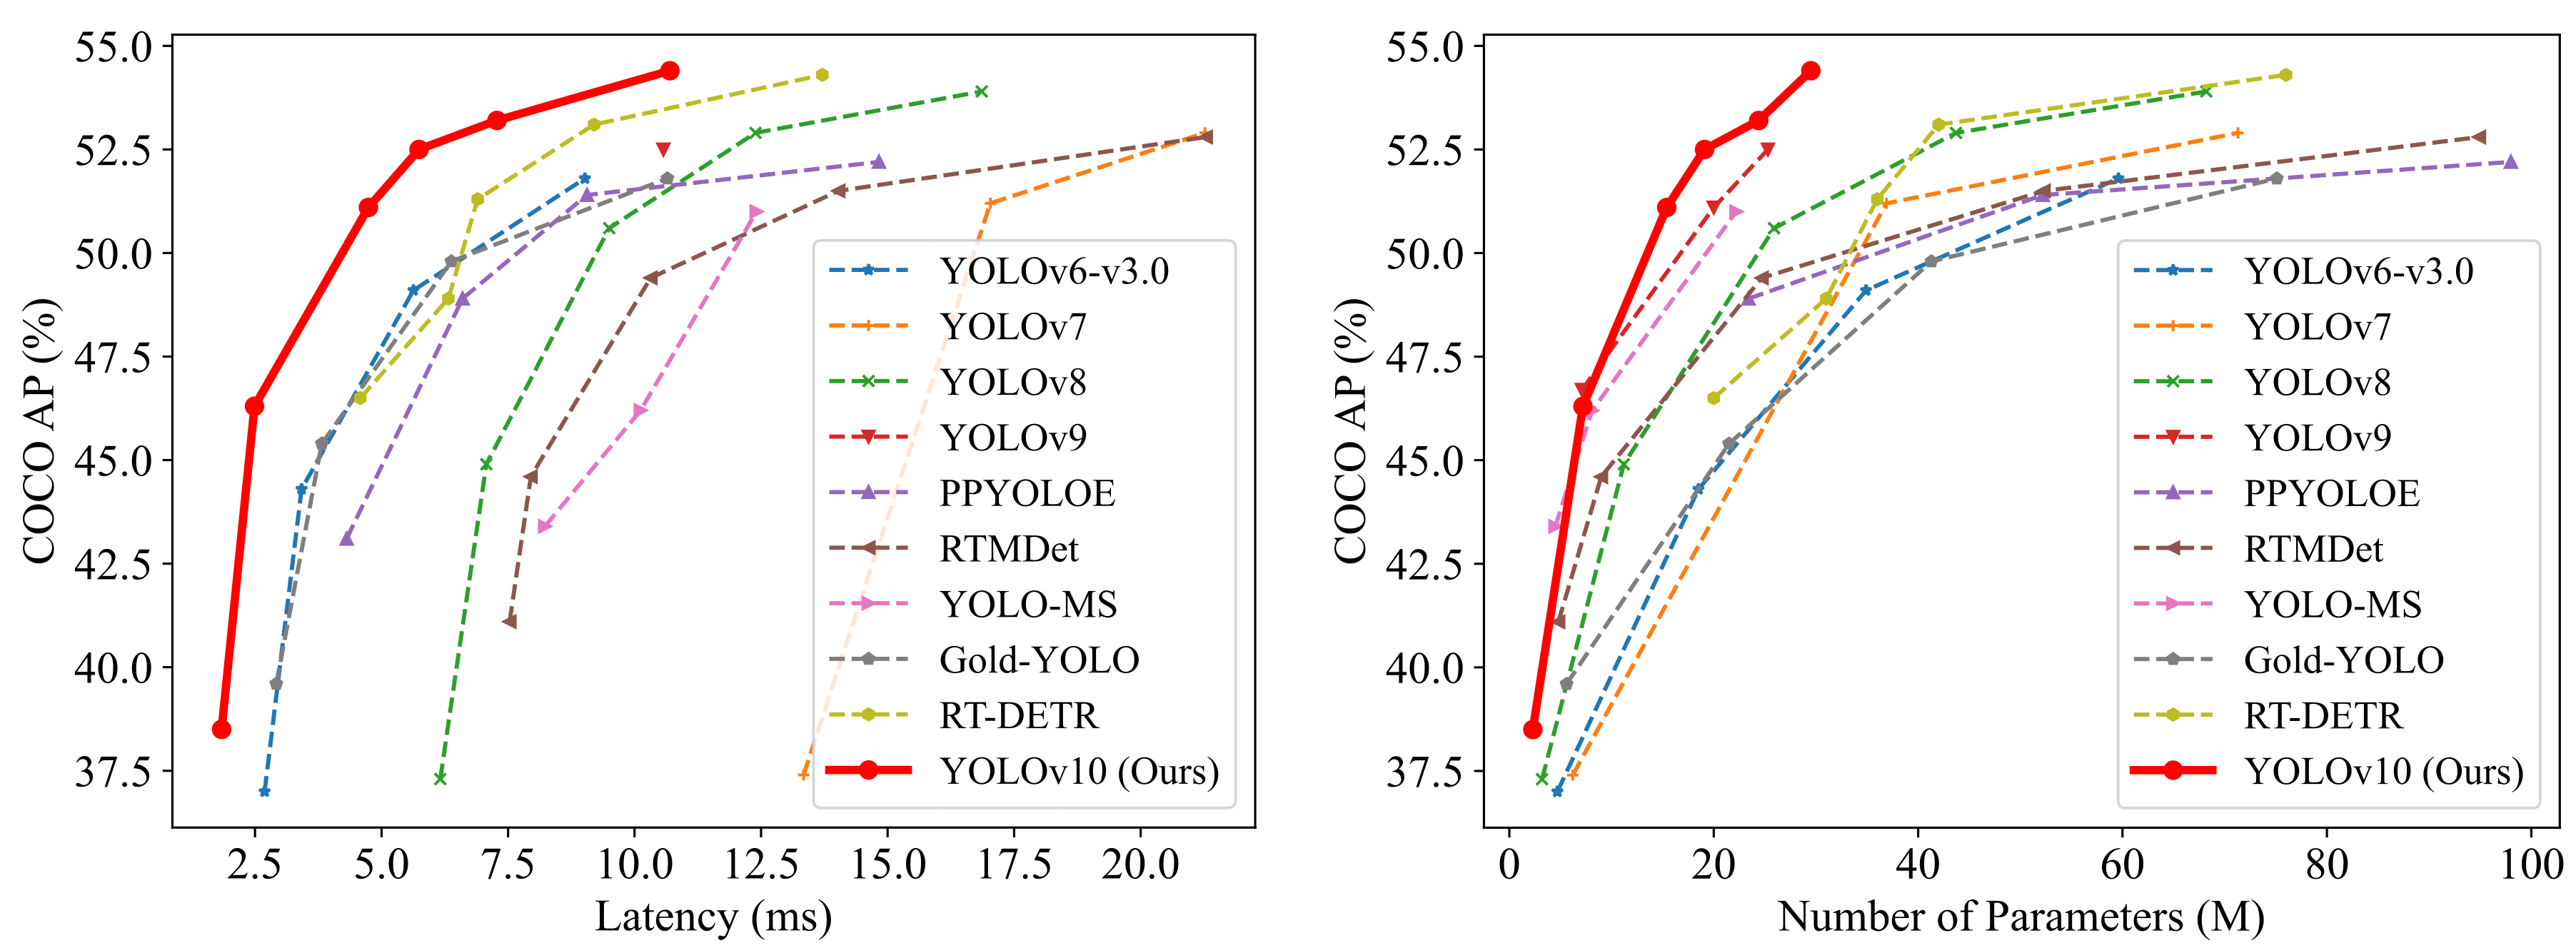
\includegraphics[width=0.8\textwidth]{figures/yolov10comp.png}
            \caption{Comparision of various models including the YOLO models v6 to v10 (https://docs.ultralytics.com/models/yolov10/)}
            \label{fig:yolo_comp}
        \end{figure}
    \subsection{Mediapipe by Google}
        MediaPipe is an open-source framework developed by Google that enables cross-platform, customisable ML across live and streaming media. It is designed to be highly flexible and to be easily integrated into a range of applications. MediaPipe provides the most complete solution for pose estimation, which is realised through a two-stage detector: first, ROI detection containing the person, then keypoint prediction inside. This methodology assists in accurate estimation of pose in real-time \citep{lugaresi2019mediapipe}. MediaPipe is very flexible; it has developed models and pipelines that can be easily customised for a developer's requirements. It supports a great variety of platforms, including Android, iOS, web, and desktop, hence making it quite accessible for various applications \citep{google2023mediapipe}. MediaPipe has been used in a host of different applications, from fitness tracking to augmented reality. On the other hand, it is a popular choice among many developers who want to implement pose estimation and several other computer vision tasks because of the capability to handle a myriad of modalities, like video or audio, and the ease of integration \citep{lugaresi2019mediapipe}. Recent improvements to MediaPipe include hand-gesture recognition by improving the framework for 3D keypoint estimation more accurately and adding support for neural network-based gesture classifiers \citep{sung2021device}.

        \begin{figure}[htbp]
            \centering
            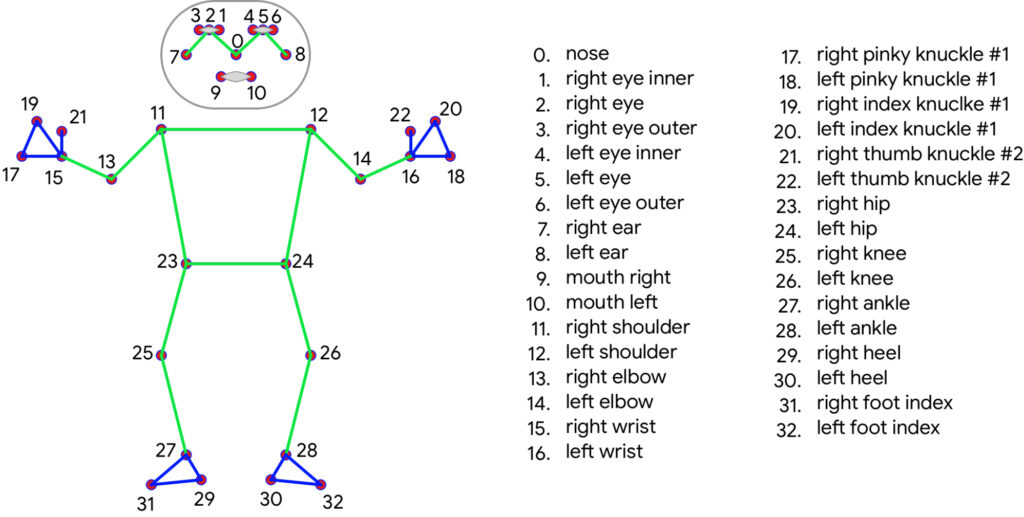
\includegraphics[width=0.75\textwidth]{figures/mediapipe.png}
            \caption{The body keypoints used by mediapipe}
            \label{fig:mediapipe}
        \end{figure}
    \subsection{Comparison}
        Let's compare these two solutions:
        \begin{enumerate}
            \item \textbf{Speed and Performance}\\
            YOLO:
            \begin{itemize}
                \item \textbf{Real-time Processing}: Models in YOLO are very fast and process natural images in real time. This makes them very appropriate to any application including immediate feedback, for example, live video analysis and autonomous systems.
                \item \textbf{Unified Architecture}: YOLO’s single-pass architecture allows it to detect objects and poses in one go, significantly reducing latency compared to multi-stage detectors.
            \end{itemize}
            MediaPipe:
            \begin{itemize}
                \item \textbf{Two-Stage Detection}: MediaPipe uses a two-stage approach: first, it detects the ROI and then predicts keypoints within the ROI. Compared with YOLO's single pass, this is slightly slower but often more accurate for pose estimation.
                \item \textbf{Optimised for Mobile and Web}: MediaPipe is designed to run efficiently on various platforms, including mobile devices and web browsers, ensuring smooth performance even on less powerful hardware.
            \end{itemize}
            \item \textbf{Flexibility and Customisation}\\
            YOLO:
            \begin{itemize}
                \item \textbf{Versatility}: In addition to position estimation, YOLO models—especially the most recent iterations, such as YOLOv8 and YOLOv10—support a variety of tasks, such as object detection, segmentation, and tracking. Because of its adaptability, YOLO is an effective tool for extensive AI vision applications.
                \item \textbf{Customisation}: YOLO allows for extensive customisation through hyperparameter tuning and integration with various frameworks, enabling developers to optimise the model for specific use cases.
            \end{itemize}
            MediaPipe:
            \begin{itemize}
                \item \textbf{Modular Design}: MediaPipe's modular architecture makes pipeline customisation and extensibility very convenient for developers to make precisely whatever application may be needed—be it a fitness tracker or an augmented reality application.
                \item \textbf{Cross-Platform Support}: MediaPipe’s ability to run on Android, iOS, web, and desktop platforms makes it highly adaptable for different deployment environments.
            \end{itemize}
            \item \textbf{Accuracy and Robustness}\\
            YOLO:
            \begin{itemize}
                \item \textbf{High Accuracy}: Accuracies of YOLO models have increased with each successive edition. For example, YOLOv10 introduces state-of-the-art techniques, such as consistent dual assignments and holistic efficiency-accuracy-driven design, to achieve state-of-the-art performance.
                \item \textbf{Robustness}: YOLO’s robust architecture and extensive training on diverse datasets ensure reliable performance across various scenarios, from crowded scenes to low-light conditions.
            \end{itemize}
            MediaPipe:
            \begin{itemize}
                \item \textbf{Precision}: The two-stage strategy of detection is very often accurate in MediaPipe pose estimation; therefore, it's applicable in various domains, from medical diagnosis to sports analysis.
                \item \textbf{Multi-Modal Capabilities}: MediaPipe’s support for multiple modalities (e.g., video, audio) enhances its robustness in handling complex tasks that require integrating different types of data.
            \end{itemize}
            \item \textbf{Ease of Integration}\\
            YOLO:
            \begin{itemize}
                \item \textbf{Integration with AI Frameworks}: YOLO models can be easily integrated with popular AI frameworks like TensorFlow, PyTorch, and ONNX, facilitating seamless deployment in various environments.
                \item \textbf{Community and Support}: The extensive community support and comprehensive documentation available for YOLO models make it easier for developers to implement and troubleshoot.
            \end{itemize}
            MediaPipe:
            \begin{itemize}
                \item \textbf{Ease of Use}: MediaPipe also provides out-of-the-box solutions and configurable pipelines, making integration easy. Also, with its intuitive API and broad reach of documentation, it empowers developers who have minimal experience in computer vision.
                \item \textbf{Google Ecosystem}: As part of the Google ecosystem, MediaPipe benefits from continuous updates and improvements, ensuring compatibility with the latest technologies and platforms.
            \end{itemize}
            \item \textbf{Use Cases}\\
            YOLO:
            \begin{itemize}
                \item \textbf{Real-Time Applications}: Ideal for applications requiring real-time processing, such as autonomous driving, surveillance, and live sports analysis.
                \item \textbf{Comprehensive Vision Tasks}: Suitable for projects that need a versatile model capable of handling multiple vision tasks simultaneously.
            \end{itemize}    
            MediaPipe:
            \begin{itemize}
                \item \textbf{Custom Solutions}: Perfect for applications that require tailored solutions, such as fitness apps, augmented reality, and interactive media.
                \item \textbf{Cross-Platform Deployment}: Best suited for projects that need to run on various platforms, including mobile devices and web browsers.
            \end{itemize}
        \end{enumerate}
        In summary, while both YOLO and MediaPipe provide very powerful tools for tasks in the estimation of human pose, the former comes short in flexibility, ease of integration, and cross-platform support. It is perfect for those applications that require bespoke solutions with seamless deployment across all platforms, thanks to its modular design and capability for handling multiple modalities. Regarding the project in this paper, MediaPipe seems the better choice.

\section{The Effect of Exercise on Mood}
    It has been known for decades that one's mental health can be improved by incorporating exercise into their lifestyle. The papers titled "The relation of physical activity and exercise to mental health." \citep{taylor1985relation} and "Psychological effects of habitual aerobic exercise: A critical review" \citep{hughes1984psychological} were early studies on this phenomenon and to what extent physical activity affects mental health. By reviewing controlled experiments on the effects of habitual aerobic exercise on mood, personality, and cognition, Tayor et al. found that the strongest evidence suggests that exercise will most likely alleviate symptoms of depression, alcoholism, anxiety, and schizophrenia, as well as improve self-image and social skills.\\
    This more recent review titled "Physical exercise and mental health: The routes of a reciprocal relation" \citep{fossati2021physical} looks at the physical-mental link in the other direction, looking to find whether this relationship is reciprocal.\\
    Finally, the study "Effects of a bout of exercise on mood in people with depression with and without physical pain" \citep{caviness2023effects} investigates the immediate effect of aerobic exercise on a community sample of 147 participants with above-average depressive symptoms by recording their mood before and after the activity. They found a statistically significant change between pre and post-workout mood.\\
    The question for this paper is: does this mood change still happen if the exercise is not aerobic, such as resistance training and callisthenics?

\section{Summary}
    Object detection, segmentation, human pose estimation, and motion tracking have all benefited from corresponding development from traditional methods up to modern deep learning frameworks. Classic techniques in the line of HOG, Haar cascades, thresholding, edge detection, and Kalman filters did much to lay the ground. Deep learning has reshaped these with R-CNN, U-Net, Convolutional Pose Machines, and LSTM networks, attaining more accuracy and efficiency. State-of-the-art solutions, such as YOLO and MediaPipe, are real-time, versatile, and cross-platform, really stretching the bounds of what could be done within computer vision.
    \subsection{Comparison of the Current Solutions}
        There are solutions to computer vision problems in terms of speed, accuracy, and suitability of applications. Most of the traditional methods are normally simple, less computationally intensive, and poor in terms of accuracy and robustness against deep approaches. Deep learning methods, like Faster R-CNN for detection and U-Net for segmentation, will rather be at the high end in terms of accuracy but at an expensive computational cost. On the other hand, YOLO models would give a compromise in speed and accuracy that is of relevance in real-time applications. MediaPipe offers flexibility and ease of integration across platforms on the other side.
    \subsection{Research Gaps}    
        While the achievements that have been made so far in this area are very inspiring, there are still some gaps in the research. The first gaps, even though this is an area which is improving, are efficient models that can run on low-power devices without a loss of accuracy. Handling of occlusions and light variation is another challenge that is currently a goal for researchers. Better generalisation across different datasets and environments, and more robust methods for real-time multi-object tracking and pose estimation in crowded scenes, are required. Addressing these gaps will be highly instrumental in taking further applications of computer vision forward.

\section{Aims \& Objectives}

% Having situated your project within a body of relevant literature, you should now be in a position to state your aims and objectives. These should be broadly similar to those given in your proposal. Most projects will have one aim that is a broad statement of what the project will achieve. The objectives should be statements of how that aim will be achieved. Objectives should be Specific, Measurable, Assignable, Realistic and Time-related (SMART).
    Based on the previous research described in the literature review above, I can know express my aims and objectives for this project. Here are the SMART goals I have set for this endeavor:

    \begin{enumerate}
        \item \textbf{Specific}: The goal of creating an AI fitness trainer application that will set the groundwork for studying the effect of exercise on mood. It involves these tasks:
        \begin{itemize}
            \item \textbf{User Detection}: Using video input to detect the presence of the user ensures the application can start analysing only when a user is present.
            \item \textbf{Keypoint Identification}: Identifying keypoints on the user's body is crucial for understanding body posture and movement.
            \item \textbf{Pose Analysis}: Analysing the poses created by the connections between keypoints allows the application to understand the user's form and make necessary inferences about occluded keypoints.
            \item \textbf{Form Recommendations}: Providing recommendations to improve the user's form help in minimising injury risks and maximising exercise effectiveness.
            \item \textbf{Mood Tracking}: Collecting the mood of the user before and after the exercise session.
            \item \textbf{Potential Add-on}: Developing a smartphone application enhances accessibility and user convenience.
        \end{itemize}
        
        \item \textbf{Measurable}: The success of the application can be qualitatively measured through:
        \begin{itemize}
            \item \textbf{Detection Accuracy}: The ability to accurately detect the human shape and keypoints. This is quantitatively measurable through metrics such as balanced accuracy, f1 score, precision, recall...
            \item \textbf{User Feedback}: Collecting user feedback on the effectiveness of the recommendations provided by the application. This is a more qualitative measure as the users' feedback will take the form of reviews. The users can be asked to give scores for usability and perceived effectivness.
        \end{itemize}
        
        \item \textbf{Achievable}: This project is achievable due to several factors:
        \begin{itemize}
            \item \textbf{Experience}: I have previous experience with image processing using Python providing a solid foundation for developing this application. As during my MComp degree, I worked on a project that detected and tracked seabirds on timelapse images using YOLOv5, tracking the birds from egg to adult stage. 
            \item \textbf{Existing Technologies}: By leveraging existing libraries and frameworks for computer vision (e.g. OpenCV, MediaPipe) can accelerate development.
            \item \textbf{Incremental Development}: By breaking down the project into smaller, manageable tasks ensures a steady progress and allows for iterative improvements.
        \end{itemize}
        
        \item \textbf{Relevant}: The project is highly relevant for several reasons:
        \begin{itemize}
            \item \textbf{Health and Fitness}: With the growing emphasis on physical and mental health and fitness, an AI personal trainer can provide valuable assistance to users looking to improve their exercise routines.
            \item \textbf{Injury Prevention}: Proper form is crucial in preventing injuries during exercise, and this application can play a significant role in educating users.
            \item \textbf{Technological Advancement}: This project contributes to advancements in AI and computer vision, showcasing practical applications of these technologies. This also creates a framework on which future research on the effect exercise as on mental health.
        \end{itemize}
        
        \item \textbf{Timebound}: The project has a clear deadline of August 29th, 2024, providing a two-month timeframe. This is sufficient for:
        \begin{itemize}
            \item \textbf{Initial Development}: Completing the core functionalities of user detection, keypoint identification, and pose analysis.
            \item \textbf{Testing and Refinement}: Conducting thorough testing and refining the application based on feedback.
        \end{itemize}
        
    \end{enumerate}  
